\chapter{Schlussfolgerung}

\section{Ergebnis}
Wenn wir unsere Programm auführen erhalten wir folgende Ausgabe:

\begin{figure}[h]
    \begin{center}
        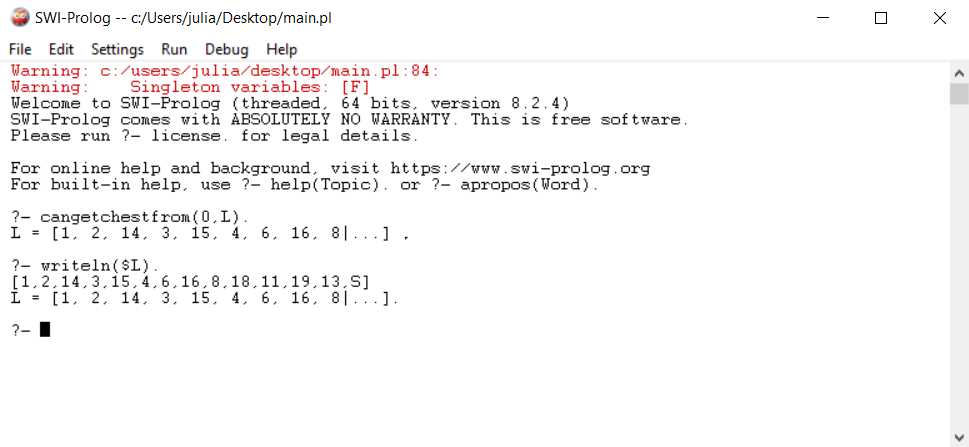
\includegraphics[width=1\textwidth]{content/pictures/output.png}
        \caption{Output Prolog Keys and Doors}
        \label{fig:output}
    \end{center}
\end{figure}

\noindent
Wie auf der Abbildung zu erkennen ist, braucht der Agent genau 13 Schritte bis
er beim Schatz angekommen ist. Dies ist nur eine von mehreren Lösungen, welche 
das Programm haben könnte.

\section{Fazit}
Es war interessant einmal mit einer Sprache zu programmieren, welche auf einem anderen Konzept basiert.
Für uns war es etwas schwierig kein, da der Programaufbau auf Rules, Facts und Queries basiert.
Dies ist ganz anders als wir es uns von Sprachen wie Java oder Python gewöhnt sind. Es hat deshalb
ein wenig Zeit gebraucht um mit Prolog klar zu kommen.
Die Sprache hat ihre Eigenheiten und muss zuerst gut kennengelernt werden, bevor man mit der
Programmierung beginnt.  